% !TeX encoding = UTF-8
\documentclass{thesisby}
\usepackage{etoolbox,ifxetex,ifluatex}

%%% Проверка используемого TeX-движка %%%
\usepackage[unicode,colorlinks=false]{hyperref}

\ifboolexpr{bool{xetex} or bool{luatex}}{%
	\PassOptionsToPackage{no-math}{fontspec}    % https://tex.stackexchange.com/a/26295/104425
	\usepackage{polyglossia}%[2014/05/21]        % Поддержка многоязычности
	% (fontspec подгружается автоматически)
	% fonts and languages
	%	\setmainfont{CMU Serif}
	
	\defaultfontfeatures{Ligatures=TeX,Mapping=tex-text}
	
	\setmainlanguage[babelshorthands = true]{russian}
	\setotherlanguage{english}
	
	%	\setmainfont{Times New Roman}
	%	\setromanfont{Times New Roman} 
	%	\setsansfont{Arial} 
	%	\setmonofont{Courier New}
	
	\setmainfont{Times New Roman}
	\setmonofont{Courier New}
	\setsansfont{Arial}
	
	\newfontfamily\cyrillicfont[Script=Cyrillic]{Times New Roman}
	\newfontfamily\cyrillicfontsf[Script=Cyrillic]{Arial}
	\newfontfamily\cyrillicfonttt[Script=Cyrillic]{Courier New}
	
	\newfontfamily\englishfont{Times New Roman}
	\newfontfamily\englishfontsf{Arial}
	\newfontfamily\englishfonttt{Courier New}
	
	\renewcommand{\UrlFont}{\small\rmfamily\tt}
	
}{%
	\usepackage[T1,T2A]{fontenc}
	\usepackage[utf8]{inputenc}
	\usepackage[english, russian]{babel}
	\IfFileExists{pscyr.sty}{\usepackage{pscyr}}{}  % Подключение pscyr
}


% Управление колонтитулами
% \headsep = 3mm
% \fancyhead{}
% \fancyfoot[C]{\thepage}

%для борьбы с переполнениями за счет разреженных слов в абзаце
\emergencystretch=25pt

\usepackage{amsmath,amssymb,amsfonts} 
\usepackage{longtable,array}
\usepackage{graphicx,epsfig}
%\usepackage[unicode,colorlinks,pagebackref]{hyperref}
%\usepackage{refcheck}% checks lost and useless labels, shows `keys' of \label in the margins

\usepackage{textcomp}% For Celsium sign only

% \graphicspath{{fig/}}
\begin{document}


\hypersetup{
pdftitle = {Руководство по оформлению диссертации с использованием \TeX овского стиля {\itshape thesisby}},
pdfauthor = {Петров Вадим Александрович},
pdfsubject = {Диссертация},
pdfkeywords = {ТеХ, диссертация}
}% End of hypersetup

\begin{titlepage}

\begin{center} \bfseries
 ������������ �������� ���� ��������\\
\bigskip
{��������������� ������� ����������}
\medskip

{<<������������ �������� ��������������
� ������� ������������ � �����>>}
\end{center}
\medskip

\noindent �� ������ ��������\\
���  123.456 \\
\vspace{1cm}

\begin{center}
{\large ������ \\ ����� �������������}\\ \vspace{1cm}

{\bfseries ����������� �� ���������� ����������� � �������������� \TeX ������� ������ {\itshape thesisby} ������ 1.0}\\
\vspace{2cm}
����������� �� ��������� ������ �������\\
��������� ���. - \TeX{} ����\\
\medskip

�� ������������� 12.34.56 \TeX ���� 
\end{center}
\vspace{3cm}

\begin{tabbing}
\hspace{8cm} \= \kill \>
������� ������������ \+ \\
�-� ���. - \TeX{} ����, ���������\\
������ �.�.
\end{tabbing}
\vspace{5cm}

\begin{center}
 \bfseries ����� 2012
\end{center}

\end{titlepage}
\tableofcontents

\newpage
\chapter*{��������}
\addcontentsline{toc}{chapter}{��������}

������ ����������� ������ ����� ����� ���������� ������������� �������� ������������ \TeX ������� ������ {\itshape thesisby} ������ 0.8 ���  ���������� ����������� � ������������ � �����������  �� 24 ������� 1997 �. $\No$ 178 � ����������� � ������������ $\No$�7/603 �� 09.03.2006~�. � $\No$�7/743 �� 03.09.2007~�. ����������� � ���������� ��������. � ��� ���� �������� ������������, ������� ����� ��������� ��� ����, ����� ���� ����������� ��������������� ����������� �����������. ����� �������� ��� ��������, ������� ����� ����������� ��������� ���������� �����������. � ������ ����������� �������������� �������������� ���������� ������������ � \TeX ��, � ����� ������ ������������ ��������� ��� �������������.

������� ��������, ��� ������ ����������� ��������� � �������������� ������������ ������ {\itshape thesisby}. ������� � ������������� ���� ���������������� ����������� ����������� ���������� � ������������� ������� ������. ������ � ����� ������� � ������, ������� ��������������� � �����������, ��������� \TeX{} ��� ������� �����������, ������� ����� ���� ����������� ��� ����� �����������.

��������� ������� ������ �������������� � ��������� ����������: http://community.livejournal.com/thesisby/.

��� �������� ������� ������ ��� ����������� �������� ��� ������ {\itshape dissert.cls} (�����: ������ ���������), ������� ��� ��������� ��� �������������� ����������� �����������. ����� ����� ���� ���� ����� �� ������ {\itshape G7-32} (�����: ������� �����). 

������ ����������� ������� �������� ��������� ����������� ������������. �� ������ �������������� �� �/��� �������������� � ������������ � ��������� ������ 2 ���� �� ������ ������ � ��������� ����� ������� ������ ����������� ������������ �������� GNU, �������������� Free Software Foundation. 

�� �������������� ������ ��������� � ������� �� ��, ��� ��� ����� ��� ��������, ������ �� ������������� �� ��� ������� ��������, � ��� ����� ����������� ��� ������������� � ���������� �����. ��� ��������� ����� ��������� ���������� ������������ �� ����������� ������������ ��������� GNU.

\newpage
\chapter{������ �����������}

\section{���������}

����� {\itshape thesisby} ����������� ����������� ���� ������ {\itshape thesisby.cls} � {\itshape longtabledef.tex}. ������ � �������� ��������������� �������, � ������ ������������ � ������ ������������� ������ � ������� ����������� ����� (��. ��������� \ref{sec:ltable}). ����� ������ {\itshape thesisby} ��� ���������� ��������� �������������� �����  ������� � ��������� ������ ������� ���������� \verb|\documentclass[rus]{thesisby}|, ��� �������� {\itshape rus} ������������� ������� ���� ��� ����������� �������� ���� � ��������. ��� ������������ ����� ������� ������������ �������� {\itshape bel}.

��� ������ � ������� ��� ����� {\itshape thesisby.cls} � {\itshape longtabledef.tex} (���� �� ���������) ������ ��������� � ����� ����� � \TeX ������ ���������� ���� ����������� ������� �������� ���������� � ����������.

����� � ��������� ����� ������������ ���������� ��� ����������� �������: {\itshape inputenc} (���������), {\itshape babel} (��������� ������), {\itshape graphicx} (������ � ��������), {\itshape array} (������� ����������� ������ � ���������), {\itshape longtable} (������ � ��������� ����������� ��������� �������), {\itshape amsmath, amssymb, amsfonts} (�������������� ������). ��� �����, ������� � ���������� � ��������� ���������� � �������� ��������, ������� ��� ������ � ������� �� ��������� ����������� ������ {\itshape indentfirst}.

\section{��������� ����, ���������� � ������������ ����� �����������}

��������� ���� ����������� � ��������� \verb|titlepage| � �������������� ����������� ��������� \verb|center| (��� �������������) �
 \verb|tabbing|(��� �������� ������ �������������� �� ��������), ������ ��� ���������������� \verb|\hspace|, \verb|\vspace|, \verb|\bigskip, \medskip, \smallskip| � ���������� ��� ���������� ���������������� ������ \verb|\large, \bfseries|.

���������� ���������� �������������� ���������� � �������� ������� \verb|\tableofcontents| � ���������� ��������� �������� ������������ ���� � �������� (����� ��� ��������, ����� �������������� ������ � ����������) ����������� ������� \verb|\addcontentsline{toc}{��� ������}{�������� �������}|, ��� ������ �������� ��������� ��� �����, � ��������� �� ��������. ��� ���� ���� ����� ���������� �������� ������ ��������������� �� �����������, ��������, \verb|\chapter*{}|.

\newpage
\chapter{����������� ����������� ������}

\section{�����, �������, ���������� � ������}

����� ���������� �������� \verb|\chapter{}|, ������� � ���������� \verb|\section{}| � \verb|\subsection{}|, ��������������, � ������, � ���� �������, �������� �������� \verb|\subsubsection{}|.

\subsection{������ ����������}

\subsubsection{������ ������}

����� ������.


\section{������� � ���������}

��� ���������� ������ � ��������� ������������ ����������� ����������� \LaTeXe. �� ��������� �������������� ������������� � �������� �����, ��� ����� ������������������ ����. 

��� ��������� �������� �������� � �������� �������������, �������� � ������� ��� ��������� ������������ ����������� ��������� \verb|eqrem|, � ������� �������� �������� � ������������� ���������� ���� �� ������� ��������~\verb|\\&|.

���� �������� ���������� ������
\begin{equation}\label{eq:H}
H_0 = \frac{p^2}{2 m} + a_0\, x^4 - a_2\, x^2,
\end{equation}
\begin{eqrem}
$p$ -- ������� �������,\\
& $m$ -- ����� �������,\\
& $x$ -- ���������� �������,\\
& $a_0, a_2$ -- ��������� �������.
\end{eqrem}

� ��� ��� ����� �������
\begin{align}
H^0_{m\, n} & = \delta_{m + 4 \; n} \;\frac{a_0 g^2}{4} \sqrt{(m + 1)(m + 2)(m + 3)(m +
4)} \notag\\
 & + \delta_{m + 2 \; n} \;\frac{g}{2} a_0  (2 m + 3) \sqrt{(m
+ 1)(m  + 2)}.
\end{align}
\begin{eqrem}
$g = \frac{m}{a_0}$ -- �������� �����������.
\end{eqrem}


\section{�������}

���� �������� �������, ������� �������� � ������������ � ������������ ���� 7.32-2001.

\begin{figure}[h!]
\begin{center}
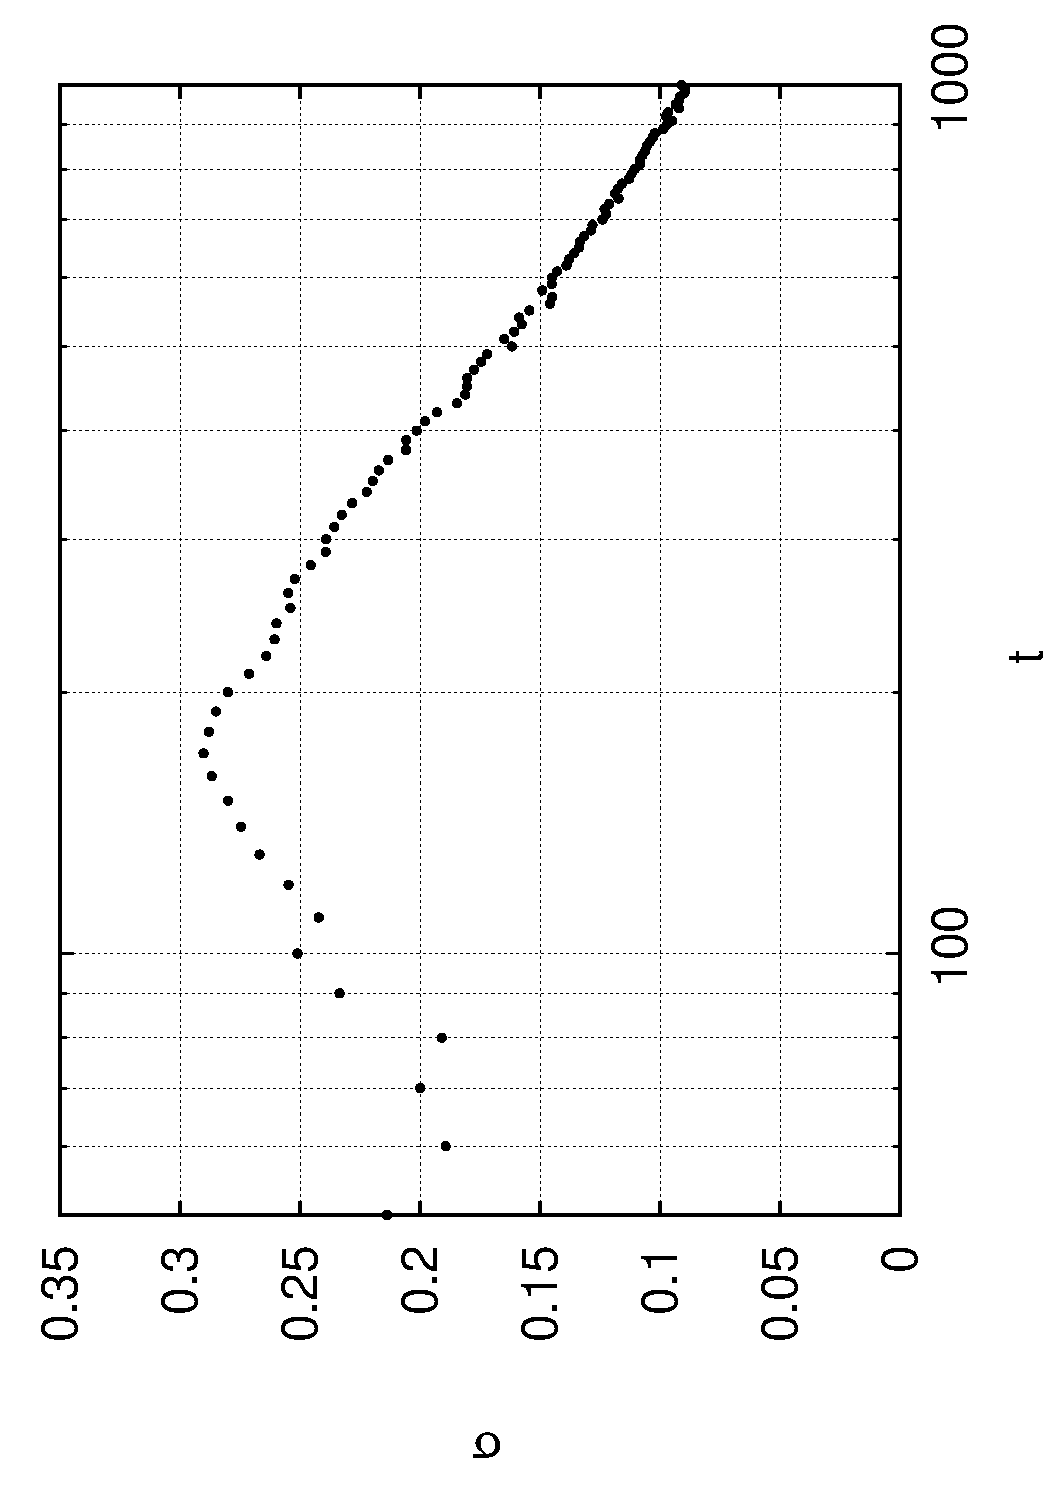
\includegraphics[angle=270,width=10cm]{test}\\[2mm]
{\small ������������� �����. ������������� �����}
\caption{������� � �������. �������������� ����������}\label{fig}
\end{center}
\end{figure}

������� ����������� � �������������� ������������ ��������� \verb|figure|, ������� ������������ ��� �������������� ���������. ������� � ������� ����������� ��� ������ ����������� ������ \verb|\includegraphics| � \verb|\caption{�������}|, ��������������, � ������������� ����� ����� ���������� ����� ������� � ����� ������ ������ ����������� � ����������� \verb|\small|. ��� ����, ����� ��������� ������ ����� �������� � ������������� ������� ����� ����� ������� ������� ������� (\verb|\includegraphics|) ��������������� �������� �������� �� ����� ������ �� �������� ��������������� ������������� ������� \verb|\\[len]|, ��� {\itshape len}--  ������ ��������������� �������.


\section{������ � ���������}

\subsection{������� �������}

��� �������� ������ ������������ ��������� \verb|table|, ������� ������������ ��������� � �������� ���������. ��� ��������� ��������� ��� �������� � ������ ���������� ��������� ���������� ������ ������� \verb|\capition{}|. ���� ������� ����� ����������� � ������� ������������ ��������� \verb|tabular|. ������ ������� �������� ���� (������� \ref{tab:1}, ��. �������� ���).

\begin{table}[h]
\caption{�������������� ��������� ������������ ������� �� ���������������}
\label{tab:1}
\begin{center}
\begin{tabular}{|l|c|c|}
\hline
������������ ����������� & ������� & ������� \\
\hline
������������ ��������� �������, \% &12 &80\\
\hline
����������� ������������ �����, \textcelsius &50 &20\\
\hline
������������ ��������� �����������, \% &100 &30\\
\hline
\end{tabular}
\end{center}
\end{table}

� ����������� ����������� ������������� � ������� ������, ������� �� 1-2 ������ ������, ��� � ��������� ������. ��� ���������� ������ ����������� ���������� ���������� ����� {\itshape array} � ��������� ������� \verb|>{\small}| ����� ����������� ��� ������� � ��������� ��������� \verb|tabular|. ������ ������������� ������ ������� ��� ������� \ref{tab:1} �������� � ������� \ref{tab:2}.

\begin{table}[h]
\caption{����������� ���� ������� � ������� ����������� �� 2 ������}
\label{tab:2}
\begin{center}
\begin{tabular}{|>{\small}l|>{\small}c|>{\small}c|}
\hline
������������ ����������� & ������� & ������� \\
\hline
������������ ��������� �������, \% &12 &80\\
\hline
����������� ������������ �����, \textcelsius &50 &20\\
\hline
������������ ��������� �����������, \% &100 &30\\
\hline
\end{tabular}
\end{center}
\end{table}

\subsection{������� � ������� ����������� �����}
\label{sec:ltable}

������� ������ � ������� ����������� ����� �� ��������� ���� ������ ����������� � ������� ��������� \verb|longtable|, ������� ������������ ������ ��������� \verb|table| � ������� ����������� ������ {\itshape longtable}. ��� �������� ��������� � ���������� ��������� ������������� ������������ ����� ���������� � ������ ��������� (����� \verb|\begin{document}|) �������� ���� {\itshape longtabledef.tex} �������� \verb|\include|. � ���������� \ref{app:table} �������� ������ ����� �������.

��� ����������� ���������� ��������� � �������� � ������� ���������� ������������ ������� \verb|\endfirsthead, \endhead, \endfoot,\endlastfoot| (��. \cite[������ 12.5]{Kotelnikov}). ��������� ��� ������ ������ ������� ����������� � �������������� ����������� ������� \verb|\caption{}|, ������� �������� ����� �������� \verb|\endfirsthead|. ��� ������� ������� ������� ������ ���� �������� ``����������� �������'' � ��������������� �������. ��� ���������� ����� ���������� ���������� ����� �������� \verb|\endhead| ����� �������� ������� ������� �������� \verb|\multicolumn{ncols}{l}{����������� ������� \ref{tableref}}|, ��� {\itshape ncols}-- ����� ������� � �������, {\itshape tableref} -- ������ �� ����� �������, ������� ����� ������ � ������ ��������� \verb|longtable| (��. �������� ��� ��� ���������� \ref{app:table}).

\subsection{������� � ������� ����������� ����}
\label{sec:gtable}

������� � ������� ����������� ����, �������� ��������, ����� ���� ������� �� �����  � �������� � �������� �������� ���� ����� ��� ������. ������ ����������� ����� ����������� ��������� ����������� �������� \LaTeXe{}  � ��������� \verb|table|. ��� ����� ������ ��������� ����� ������� ����������� � �������������� ��������� \verb|tabular|. ��� ������ ������ ������� �������� (������������ \verb|\caption{}|), � ��������� ����� ���������� ��������� ������������ �������� \verb|\smallskip| ��� \verb|\medskip| � ������������� �������� �����������. ������ ����� ������� �������� � ����������~\ref{app:gtable}.

\section{����������}

� ������ ������ ���������� ����������� ���������� ���������� ��� ������ ��������� \verb|comments| � \verb|comment|. � ������ �������������� ������� ���������� ����������, ������� ���������� �������� \verb|\item|, � ������ ������������� ��� ��������� � ����� ���������� ���������� ��� ���������. ������� �������� ������ ��������� \verb|comments|:

\begin{comments}
\item ����� ������� ������ ������� ����������. ����� ������� ������ ������� ����������. ����� ������� ������ ������� ����������. ����� ������� ������ ������� ����������. ����� ������� ������ ������� ����������.

����� ������� ������ ������� ����������. ����� ������� ������ ������� ����������. ����� ������� ������ ������� ����������. ����� ������� ������ ������� ����������.

\item ����� ������� ����������. ����� ������� ����������. ����� ������� ����������. ����� ������� ����������.
\end{comments}

� ������ ��������� \verb|comment|:
\begin{comment}
����� ����������. ����� ����������. ����� ����������. ����� ����������. ����� ����������. ����� ����������. ����� ����������. ����� ����������. ����� ����������. ����� ����������. ����� ����������. ����� ����������.

����� ����������. ����� ����������. ����� ����������. ����� ����������. ����� ����������. ����� ����������. ����� ����������. ����� ����������. ����� ����������. ����� ����������. ����� ����������. ����� ����������. ����� ����������. ����� ����������. ����� ����������.
\end{comment}

�� ����������� ���� �������� ����� ������� � ���������� ���������� ���� ���������.


\chapter{���������� ������������}

� ��������������� ������ ������������ ����������� ��������� \verb|thebibliography| ��� ���������� ������ �������������� ���������� � ����������� ��� ��������� \verb|mybibliography| ��� ������ ���������� ����������. � ������ ����������� �������� ������ ���������. ���� ��������� ����������� � �������������� ������� �������� ����������������� ������ \verb|\bibitem{}|, � ������ � ������ ����������� � �������������� ����������� ������� \verb|\cite{}| ��� �� ����������� ����� \verb|\cite[]{}|, ���� ���������� ������� �������������� ���������� ��� ������� ���������.

�������� ��������� �������� ������. ������� ������ �� �������������� ��������� \cite{Kotelnikov,article} � 
\cite{proc}. ����� ������� ����� ��������� ��� \cite[�. 25]{Kotelnikov} � \cite[������� 2]{article}. � ������ ������ �� ������������ ������ ���������� \cite{myarticle,myproc}  � �� ������������� ������ � ����� ������� ���� \cite[�������~4]{myrussianarticle} � \cite[�����~2]{mybook}.

��� �� ������� �������� �������� �� ��, ���, � ������ ������������� ���������� ������ ���������� �� �����, ������ ������������ ���������� ��� �������� ������������ BiBTeX (��. \cite[����� 13]{Kotelnikov}). ���������� ����������� ����������������� �������� �����, ������� ��������� ��������� ������������ � �������� � ������������� ����������� ������������. ��� ����� {\itshape gost780s.bst} � {\itshape gost780u.bst}, ��������������, � ����������� � ��� ���. �� ��� ������������� ��������� ������ � ������  ����������������� ���� ������, ������������ ������� ����, ���������� ��������� ��������� ������: \verb|language = {russian}|.

\chapter*{����������������� ������}
\addcontentsline{toc}{chapter}{����������������� ������}

\begin{thebibliography}{8}
\def\selectlanguageifdefined#1{
\expandafter\ifx\csname date#1\endcsname\relax
\else\language\csname l@#1\endcsname\fi}

\bibitem{Kotelnikov}
\selectlanguageifdefined{russian}
�����������,~�.~�. \LaTeXe{} ��-������~/ �.~�. �����������, �.~�.
  ��������. ---
\newblock 3-� {\cyr\cyri\cyrz\cyrd.} ---
\newblock ��������� ���������, 2004 (\href{http://www.tex.uniyar.ac.ru/doc/kotelnikovchebotaev2004b.pdf}{PDF document}).

\bibitem{hyperref}
\selectlanguageifdefined{russian}
���������� � PDF ����������, ��������� ���������� \LaTeXe. // �������� ������ / \TeX{} � ����  [����������� ������]. - 2002.
 - ����� �������: \href{http://www.tex.uniyar.ac.ru/doc/href\_in\_LaTeX.pdf}{PDF document}. - ���� �������: 27.11.2008.

\bibitem{hyperrefop}
\selectlanguageifdefined{russian}
����� ������ hyperref ��� ��������� PDF ������. // �������� ������ / \TeX{} � ����  [����������� ������]. - 2002. - ����� �������:
\href{http://www.tex.uniyar.ac.ru/doc/hyperref\_options.pdf}{PDF document}.  - ���� �������: 27.11.2008.

\bibitem{refcheck}
\selectlanguageifdefined{english}
Refcheck for \LaTeXe. //  The \TeX{} catalogue online  [Electronic resource]. - 2004. - Mode of access:
\href{http://www.ctan.org/tex-archive/macros/latex/contrib/refcheck/refdemo.pdf}{PDF document}.  - Date of access: 27.11.2008.

\bibitem{article}
\selectlanguageifdefined{english}
Author,~A.~A. Long title~/ A.~A. Author~// Journal name. ---
\newblock 2008. ---
\newblock Vol.~11. ---
\newblock P.~11--25.

\bibitem{proc}
\selectlanguageifdefined{english}
Author,~A.~A. Paper title~// Proceedings of the conference. ---
\newblock 2006. ---
\newblock P.~23--29.

\end{thebibliography}


% For BibTeX
% \bibliographystyle{gost780u}
% \bibliography{bibtexbase}

\begin{mybibliography}{8}
\def\selectlanguageifdefined#1{
\expandafter\ifx\csname date#1\endcsname\relax
\else\language\csname l@#1\endcsname\fi}

\bibitem{myarticle}
\selectlanguageifdefined{english}
Author, A.A. Long title~/ A.A. Author, V.A. Piatrou~//
  Journal name. ---
\newblock 2008. ---
\newblock Vol.~1. ---
\newblock P.~10--15.

\bibitem{myproc}
\selectlanguageifdefined{english}
Piatrou, V.A. My paper title~// Proceedings of the conference.

\bibitem{myrussianarticle}
\selectlanguageifdefined{russian}
������, �.�. �������� ������~/ �.�. ������~//
  �������� �������. ---
\newblock 2007. ---
\newblock \CYRT.~10. ---
\newblock {\cyr\CYRS.}~110--114.

\bibitem{mybook}
\selectlanguageifdefined{russian}
������, �.�. �������� �����~/ �.�. ������ ---
\newblock 1-�  {\cyr\cyri\cyrz\cyrd.} ---
\newblock �������� ������������, 2006.

\end{mybibliography}


\appendix
\chapter{���������� ����������}
\label{app:1}

���������� ���������� ���������� �������� ������� \verb|\appendix|, ������� �������� ����� ���������� ���������. ����� ������ �������, ������� \verb|\chapter{��������}| ������ �� ����� �����, � ����� ����������, ������� ���������� �������. ���������� ��������� � � ������ ���������, ����� ��� �������, ������� � �������, ������� ������� ��������� ���� (��. ������� \ref{app:fig}, ������� (\ref{app:eq}) � ������� \ref{app:tab}).

\begin{figure}[ht!]
\begin{center}
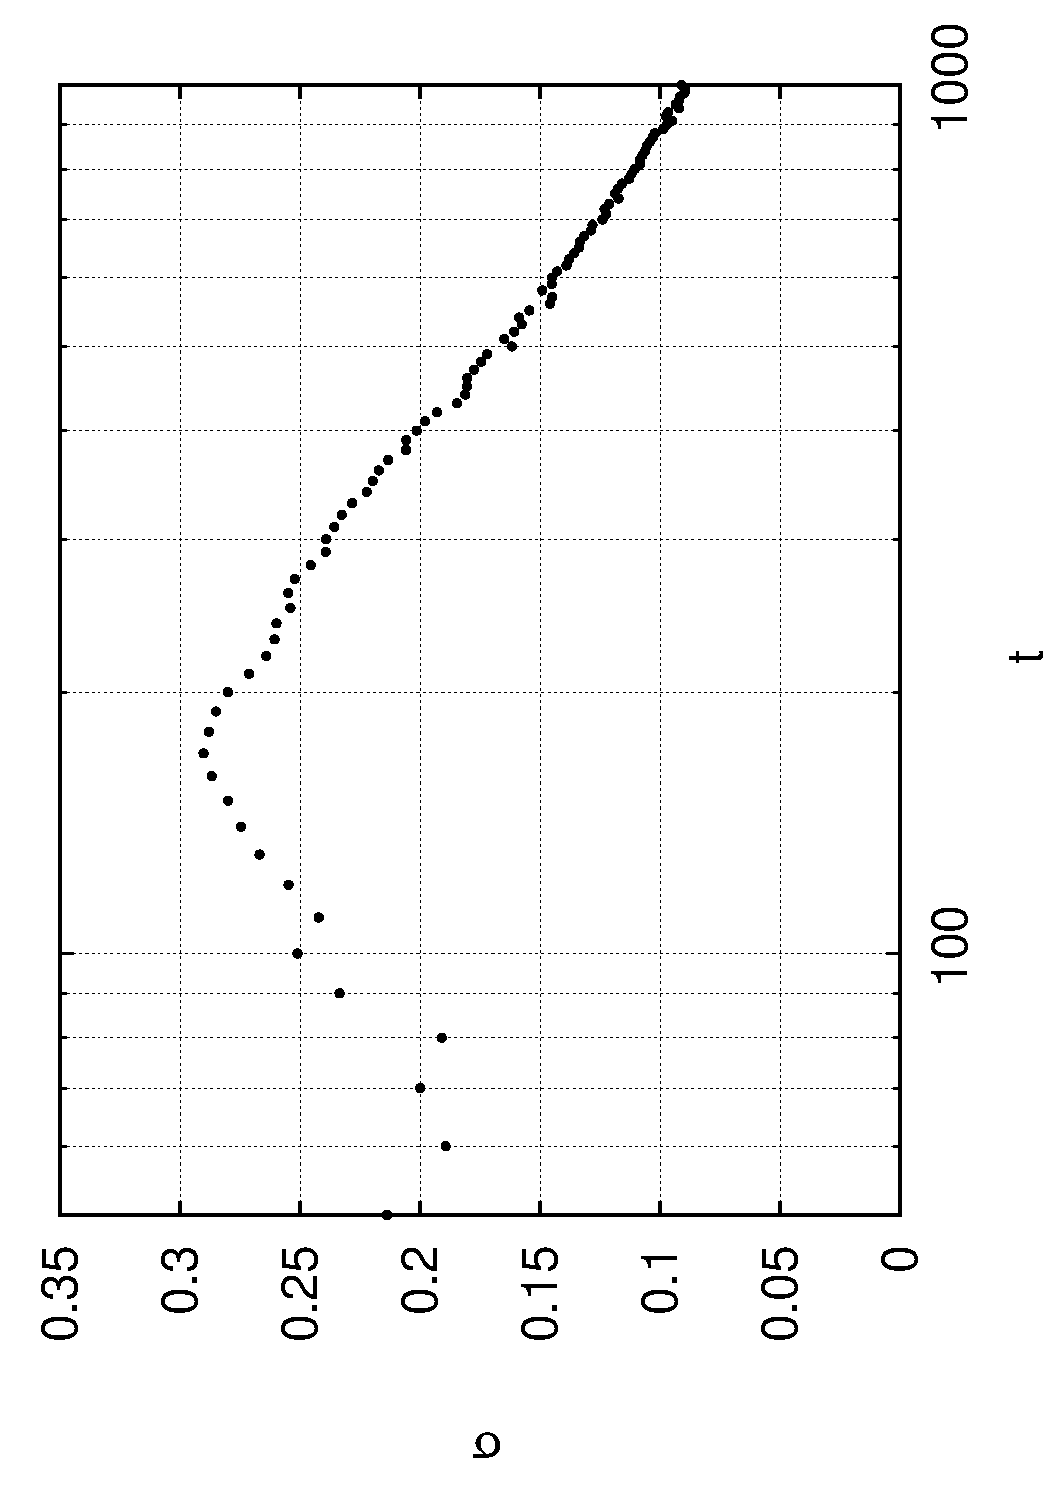
\includegraphics[angle=270,width=7cm]{test}\\
\caption{������� � �������. �������������� ����������}
\label{app:fig}
\end{center}
\end{figure}

\begin{equation}\label{app:eq}
V = x^4 - 2 x^2,
\end{equation}
\begin{eqrem}
$x$ -- ���������� �������.
\end{eqrem}

\begin{table}[h]
\caption{�������������� ��������� ������������ �������}
\begin{center}
\begin{tabular}{|>{\small}l|>{\small}c|>{\small}c|}
\hline
������������ ����������� & ������� & ������� \\
\hline
������������ ��������� �������, \% &12 &80\\
\hline
����������� ������������ �����, \textcelsius &50 &20\\
\hline
������������ ��������� �����������, \% &100 &30\\
\hline
\end{tabular}\label{app:tab}
\end{center}
\end{table}


\section{������ � ���������� \ref{app:1}}

���������� ����� ����������� �� �������, ���������� � ������ � �������������� ����������� ������ ���������������.

\chapter{���������� ������� �����������, ������������ � �����������}\label{app:template}

���� ������������ ������� \ref{table}, ������� ���� ���������� ������������� ��������� ���������� �������� �����������, ������������, ����������� � ������ ��������������� ������, ������� �������� � ������� ����� ����� ������� \verb|\include{��� �����}|.

�������� ������������� ���������� �������� ������������ ��������� ���������� ����������� ���� � �� �� ������ � ������ ����������. ��������, ��������� ��������� �� ������ ������ ������������� � �����������, ������������ � �����������. ������������� ����� \textit{statements.tex}, ������� �������� ��������� � ������������ �� ���� ��������� ���� ����������, ����������� �������� ������ ��� ������������ � ��������� ������������� ��������� ������� �� ���������������� ��������� � ������ ����������. �� �� �������� ������ �����������, ������� ����� ������ ���� � � ������������ (��������, ����� �������������� ������, ���������� � ������������ �� ������������� ������������� �����������).

\begin{table}[t]
\caption{�������, ���������� ��������� � ����� � ���������� �������� �����������, ������������ � �����������}\label{table}
\begin{center}
\begin{tabular}{|p{58mm}|p{48mm}|p{49mm}|}
\hline
\large \bfseries ����������� & \large \bfseries ����������� & \large \bfseries ����������� \\[2mm]
\hline
\multicolumn{3}{|c|}{\bfseries ������� ����}\\
\hline
\itshape THESIS.tex & \itshape ABSTRACT-PhD.tex & \itshape PRESENTATION.tex \\
\hline
\multicolumn{3}{|c|}{\bfseries ���������� �����}\\
\hline
\multicolumn{3}{|c|}{\textit{statements.tex} -- ���������, ��������� �� ������}\\
\hline
\multicolumn{3}{|p{16cm}|}{������� �������� � ����� \textit{``fig''} � pdf �������. ��������� ���������� ����� ������������ pdfLaTeX. ��� �������� LaTeXa ����� EPS �������.}\\
\hline
\textit{definitions.tex} -- ������ �����������,
\newline \textit{titlepage.tex} -- ��������� ��������,
\newline \textit{thesisintro.tex} -- ������ �����������  &  \bfseries \large --- &
\textit{beamerthemeMinsk.sty} - ����� ``�����'' ��� ����������� (����� ������������ ����� ������ �����, ��. \cite{beamer}) \\
\hline
\multicolumn{2}{|c|}{\textit{intro.tex} -- ��������} & \bfseries \large --- \\
\hline
\multicolumn{2}{|c|}{\textit{characteristics.tex} -- ����� �������������� ������} & \bfseries \large --- \\
\hline
\textit{chapter1.tex, chapter2.tex, chapter3.tex, chapter4.tex} -- ������ ����� & \bfseries \large ---   & \bfseries \large --- \\
\hline
\multicolumn{2}{|c|}{\textit{conclusions.tex} -- ����������} & \bfseries \large --- \\
\hline
\multicolumn{2}{|p{11cm}|}{\textit{recommendations.tex} -- ������������ �� ������������� ������������� �����������} & \bfseries \large --- \\
\hline
\textit{bib.tex} -- ����������������� ������ + ������ ������ & \bfseries \large ---   & \bfseries \large --- \\
\hline
\multicolumn{2}{|p{11cm}|}{\textit{bibmypapers.tex} -- ������ ���������� � ������� ��������} & \bfseries \large ---  \\
\hline
\multicolumn{2}{|p{11cm}|}{\textit{bibmyreports.tex} -- ������ ���������� � ���������� �����������} & \bfseries \large ---  \\
\hline
\textit{appendix.tex} -- ����������.  & \bfseries \large ---   & \bfseries \large --- \\
\hline
\end{tabular}
\end{center}

\end{table}


\chapter{��������� ����������}

�������� �����������, ���������� ������� ���������� ���������� ������� �������� ��������. � ������ ������ ��� ������������ ������������� ��� ������� ������� ������ ������ ���������� \verb|\chapter{�������� ����������}|. �� ����� �������� �������� �� ��, ��� �� ��� ����� ����� ���� ������������ ��� ���������. ����� �, �, �, �, �, �, �, � ������ ���� ��������� �� ���������. � ������ ������������ ������� \verb|\Asbuk| ��� ����� ������������� �������� ����������, ������� ���� �� �������� � ��������� ����� �, �, �, �, �. �� ����� �, �, �, ��������. ��� �� ���������� ����� �����������, ������� ����� �������� ������������ �����, ����� �������� ������� ���������� {\itshape chapter}, ��������� ������� \verb|\addtocounter{chapter}{1}|.

��� ��������� ���������� ����� ����� ������������ ������� ���������� ��������. ��� ����� ����� ����� �������  \verb|\appendix|, �������� ������ ����������, ����� �������������� ����� ��������: \verb|\renewcommand{\thechapter}{\Alph{chapter}}|. ���������� ������ ���� I � O �� ��������� �������������� ��������� ���� ��������.


\chapter{������� � �����\'{�}� ����������� �����}
\label{app:table}

���� �������� ������ ������� � ������� ����������� �����. �������� ���������� �� ���������� ������� ���� ������ ��������� � ����������~\ref{sec:ltable} � ����� \cite[������ 12.5]{Kotelnikov}.

\begin{longtable}{|l|c|c|}
\caption{������� � ������� � ������� ����������� �����. ������� �������� ��� ��������.}
\label{tab:long}
 \\ \hline
������� & ������ ������� & ������ ������� \\ \hline
		\endfirsthead
\multicolumn{3}{l}{����������� ������� \ref{tab:long}}
\\ \hline
������� & ������ ������� & ������ ������� \\ \hline
		\endhead
		\endfoot
	\hline  \endlastfoot

�������� & ������� ������� ������� & ������� ������� ������� \\
�������� & ������� ������� ������� & ������� ������� ������� \\
�������� & ������� ������� ������� & ������� ������� ������� \\
�������� & ������� ������� ������� & ������� ������� ������� \\
�������� & ������� ������� ������� & ������� ������� ������� \\
�������� & ������� ������� ������� & ������� ������� ������� \\
�������� & ������� ������� ������� & ������� ������� ������� \\
�������� & ������� ������� ������� & ������� ������� ������� \\
�������� & ������� ������� ������� & ������� ������� ������� \\
�������� & ������� ������� ������� & ������� ������� ������� \\
�������� & ������� ������� ������� & ������� ������� ������� \\
�������� & ������� ������� ������� & ������� ������� ������� \\
�������� & ������� ������� ������� & ������� ������� ������� \\
�������� & ������� ������� ������� & ������� ������� ������� \\
�������� & ������� ������� ������� & ������� ������� ������� \\
�������� & ������� ������� ������� & ������� ������� ������� \\
�������� & ������� ������� ������� & ������� ������� ������� \\
�������� & ������� ������� ������� & ������� ������� ������� \\
�������� & ������� ������� ������� & ������� ������� ������� \\
�������� & ������� ������� ������� & ������� ������� ������� \\
�������� & ������� ������� ������� & ������� ������� ������� \\
�������� & ������� ������� ������� & ������� ������� ������� \\
�������� & ������� ������� ������� & ������� ������� ������� \\
�������� & ������� ������� ������� & ������� ������� ������� \\
�������� & ������� ������� ������� & ������� ������� ������� \\
�������� & ������� ������� ������� & ������� ������� ������� \\
�������� & ������� ������� ������� & ������� ������� ������� \\
�������� & ������� ������� ������� & ������� ������� ������� \\
�������� & ������� ������� ������� & ������� ������� ������� \\
�������� & ������� ������� ������� & ������� ������� ������� \\
�������� & ������� ������� ������� & ������� ������� ������� \\
�������� & ������� ������� ������� & ������� ������� ������� \\
�������� & ������� ������� ������� & ������� ������� ������� \\
�������� & ������� ������� ������� & ������� ������� ������� \\
�������� & ������� ������� ������� & ������� ������� ������� \\
�������� & ������� ������� ������� & ������� ������� ������� \\
�������� & ������� ������� ������� & ������� ������� ������� \\
�������� & ������� ������� ������� & ������� ������� ������� \\
�������� & ������� ������� ������� & ������� ������� ������� \\
�������� & ������� ������� ������� & ������� ������� ������� \\
�������� & ������� ������� ������� & ������� ������� ������� \\
�������� & ������� ������� ������� & ������� ������� ������� \\
\end{longtable}
%\end{table}

\chapter{������� � �����\'{�}� ����������� ��������}
\label{app:gtable}

���� �������� ������ ������� � ������� ����������� ��������. �������� ���������� �� ���������� ������� ���� ������ ��������� � ����������~\ref{sec:gtable}.

\begin{table}[h]
\caption{�������������� ��������� ������������ ������� �� ���������������}
\label{tab:g}
\begin{tabular}{|>{\small}l|>{\small}c|>{\small}c|>{\small}c|}
\hline
������������ ����������� & ������� & ������� & ������� \textnumero 3 \\
\hline
������������ ��������� �������, \% &12 &80 &42 \\
\hline
����������� ������������ �����, \textcelsius &20 &12 &80 \\
\hline
������������ ��������� �����������, \% &100 &32 &84 \\
\hline
\end{tabular}

\smallskip
����������� ������� \ref{tab:g}\\
\begin{tabular}{|>{\small}l|>{\small}c|>{\small}c|>{\small}c|}
\hline
������������ ����������� & ������� \textnumero 4 & ������� \textnumero 5 & ������� \textnumero 6 \\
\hline
������������ ��������� �������, \% &80 &42 &83 \\
\hline
����������� ������������ �����, \textcelsius &20 &12 &80 \\
\hline
������������ ��������� �����������, \% &100 &32 &84 \\
\hline
\end{tabular}

\smallskip
��������� ������� \ref{tab:g}\\
\begin{tabular}{|>{\small}l|>{\small}c|>{\small}c|>{\small}c|}
\hline
������������ ����������� & ������� \textnumero 7 & ������� \textnumero 8 & ������� \textnumero 9 \\
\hline
������������ ��������� �������, \% &80 &42 &82 \\
\hline
����������� ������������ �����, \textcelsius &40 &12 &80 \\
\hline
������������ ��������� �����������, \% &100 &34 &84 \\
\hline
\end{tabular}


\end{table}




\end{document}